\chapter{Tehnologii folosite}
\section{Python}

Python este un limbaj de programare high-level, cunoscut pentru sintaxa sa clară și concisă \cite{van2006introduction}. A fost creat de Guido van Rossum în 1991. El este folosit pe scară largă, fiind renumit pentru aplicabilitatea lui în mai multe domenii. Printre acestea se numără dezvoltarea  web, data science, automatizarea și inteligența artificială.

Pentru crearea aplicațiilor de automatizare, Python reprezintă una dintre cele mai bune alegeri. Acest limbaj oferă mai multe avantaje deoarece prezintă o sintaxă intuitivă și o multitudine de librării, actualizate constant, care facilitează procesul de automatizare.


\section{Pip}

Pip este un manager de pachete pentru Python folosit pentru a instala și gestiona librării. Acesta permite instalarea ușoară a pachetelor din PyPI (Python Package Index) și are o sintaxă ușor de înțeles. Câteva comenzi de bază sunt:
\begin{itemize}
	\item \textbf{pip install <nume librărie>}: pentru a instala o librărie
	\item \textbf{pip uninstall <nume librărie>}: pentru a dezinstala o librărie
	\item \textbf{pip list}: pentru a afișa toate librăriile instalate
	\item \textbf{pip show <nume librărie>}: pentru a afișa mai multe informații despre o librărie
\end{itemize}


\section{PyMuPDF}

Una dintre provocările întâlnite a fost alegerea unei librării eficiente pentru manipularea documentelor PDF. Inițial, aplicația a fost dezvoltată folosind PyPDF2. Deși PyPDF2 este o librărie care manipulează documente în format PDF, aceasta s-a dovedit a fi prea lentă pentru volumul de manuale care trebuiau gestionate și nu oferea toate funcționalitățile necesare.

Pentru a depăși aceste limitări, a fost aleasă librăria PyMuPDF \cite{pymupdf}. Această librărie open-source oferă viteze mari pentru extragerea și scrierea infromațiilor din documente PDF. A fost inițial dezvoltată de Jorj X. McKie, iar ulterior a fost preluată de Artifex.

Pe lângă avantajele pe care le are această librărie în Python, PyMuPDF este disponibilă și în C și JavaScript. O diferență majoră între PyMuPDF și alte librării constă în faptul că celelalte librării sunt limitate doar la documente PDF, în timp ce PyMuPDF poate manipula o varietate de alte documente, cum ar fi XPS, EPUB, MOBI, FB2, CBZ, SVG, DOCX, XLSX și PPTX.

Conform site-ului oficial de la PyMuPDF \cite{pymupdf}, această librărie este una dintre cele mai rapide librării din Python pentru manipularea documentelor PDF. Drept dovadă, vor fi analizate cele mai importante funcționalități ale unei librării de acest fel: viteza de copiere, viteza de extragere și viteza de transformare a paginii într-o imagine.

Testele puse la dispoziție au fost realizate pe un set de 8 documente PDF cu un total de 7031 de pagini care conțin atât fragmente de text, cât și imagini.

Primul test măsoară viteza de citire si de rescriere a unui document PDF. Este un proces esențial pentru aplicațiile web ce permit combinarea mai multor documente PDF. Rezultatele testului sunt afișate în figura 3.1.
\begin{figure}[H]
	\centering
	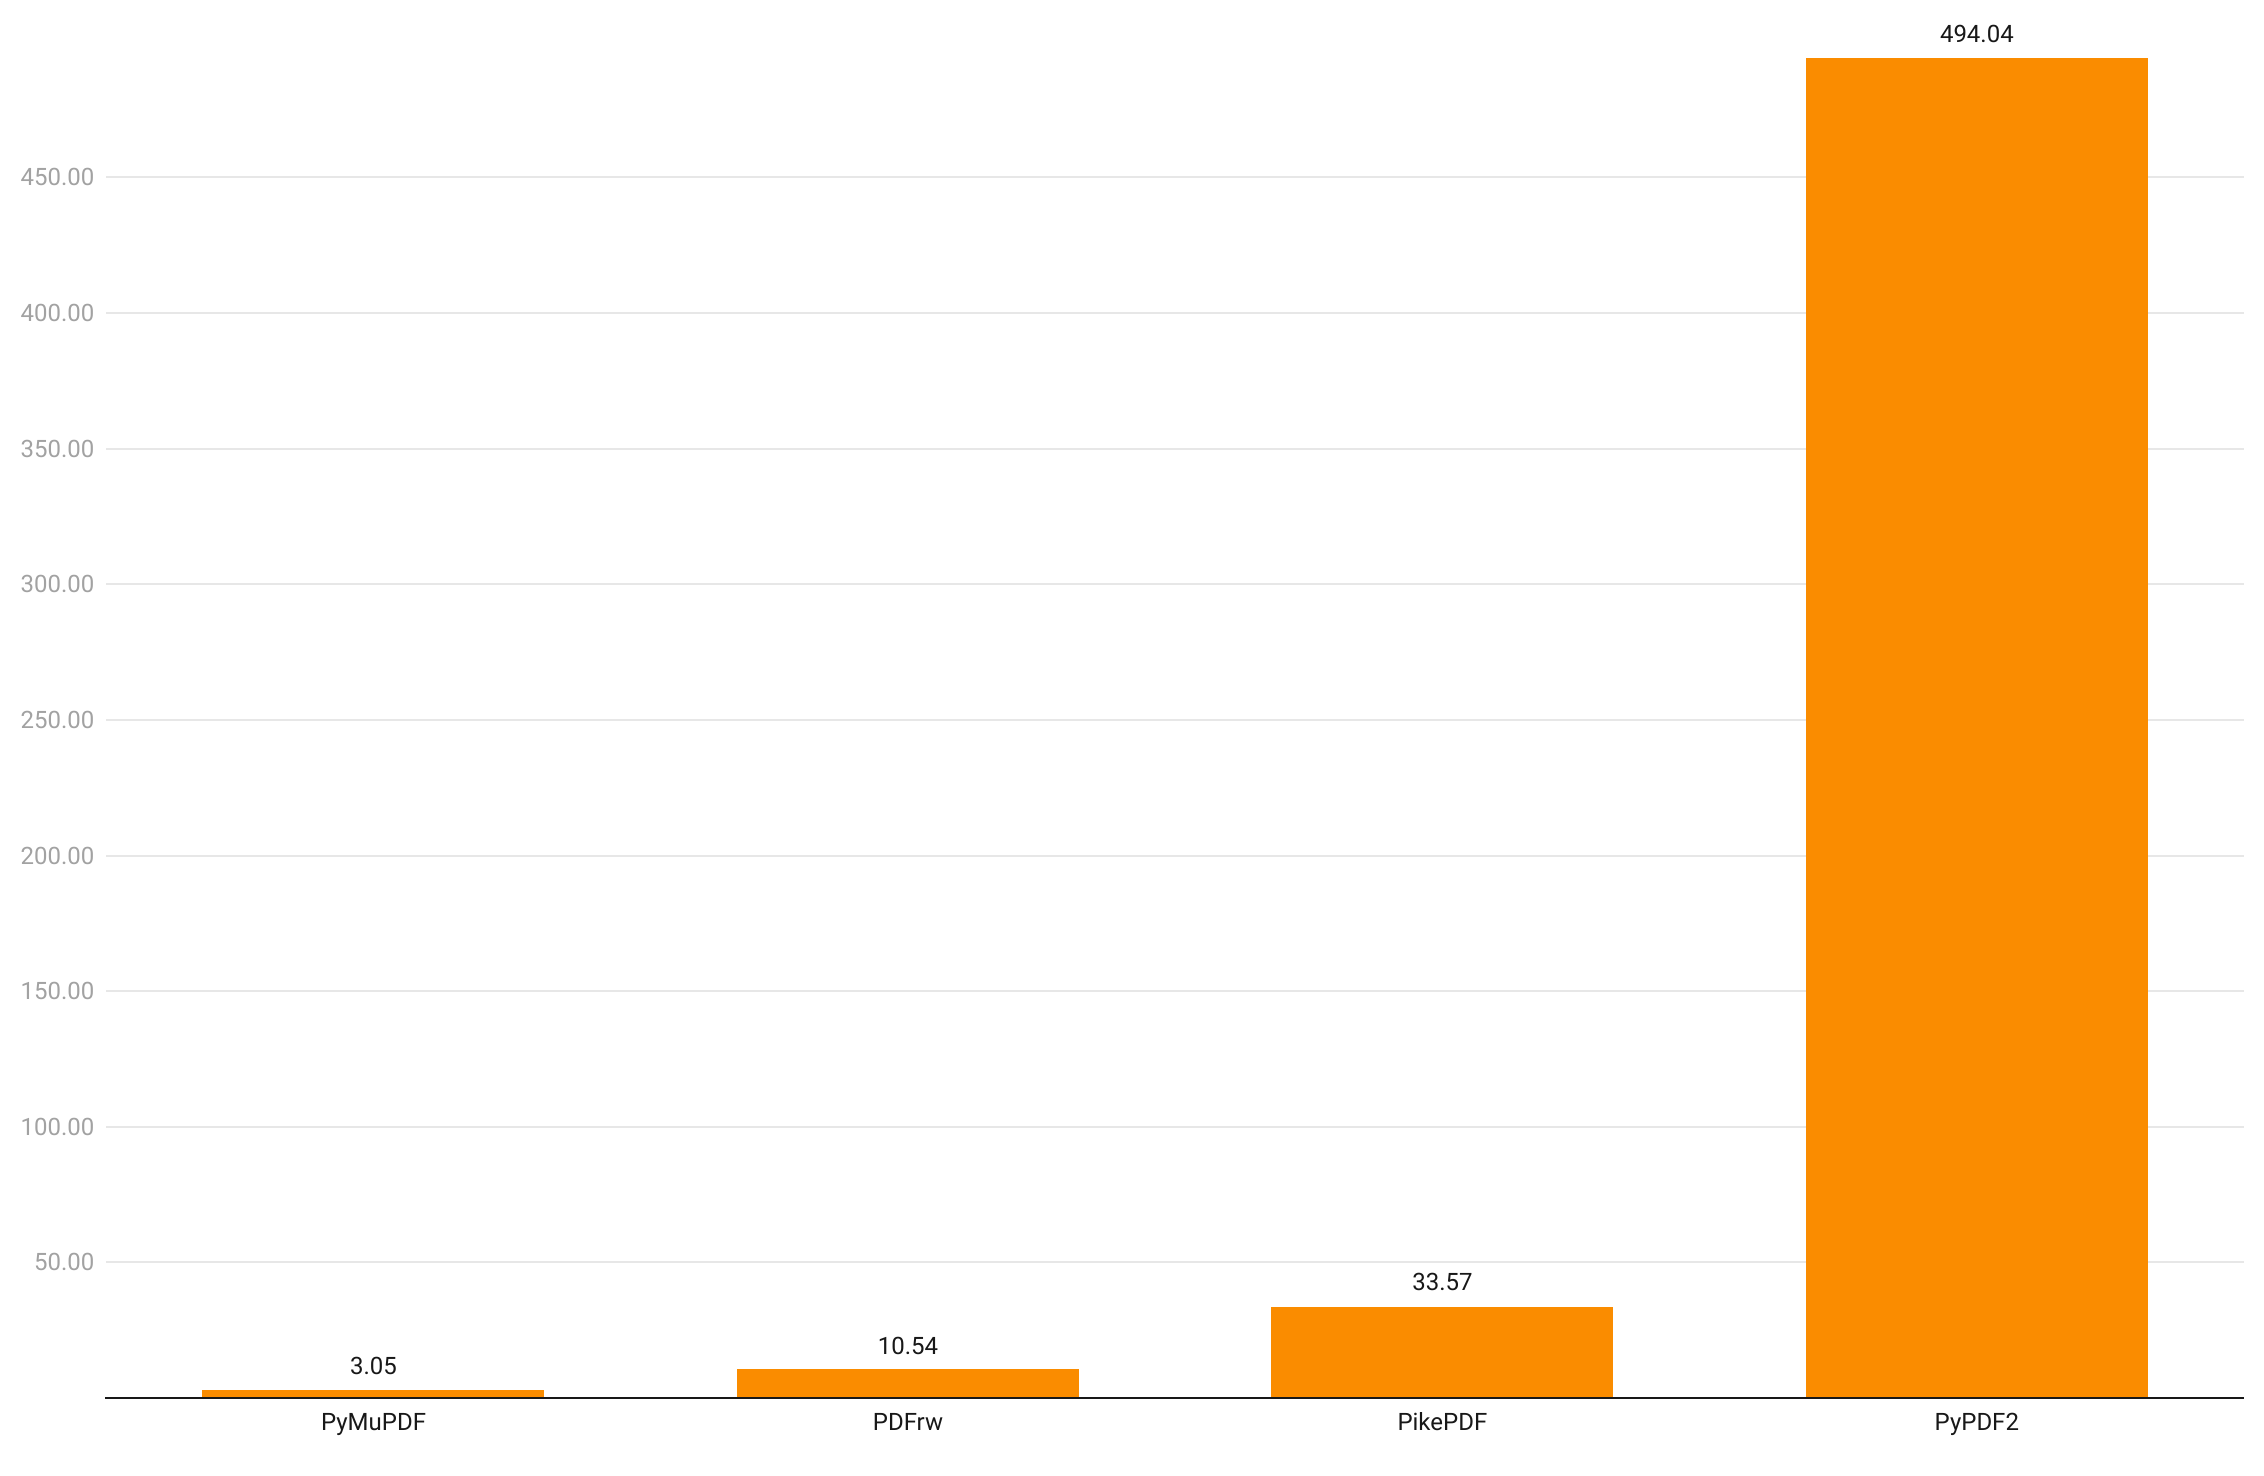
\includegraphics[scale=.25]{Figura3_1}
	\caption{Comparație de timp (în secunde) pentru copierea documentelor PDF}
	\label{fig:Figura3_1}
\end{figure}

Al doilea test măsoară durata procesului de extragere a unui text simplu dintr-un document PDF și scrierea lui într-un fișier .txt. Acest lucru este util pentru căutarea unui anumit termen din document sau pentru a efectua modificări în text. Rezultatele testului sunt afișate în figura 3.2.
\begin{figure}[H]
	\centering
	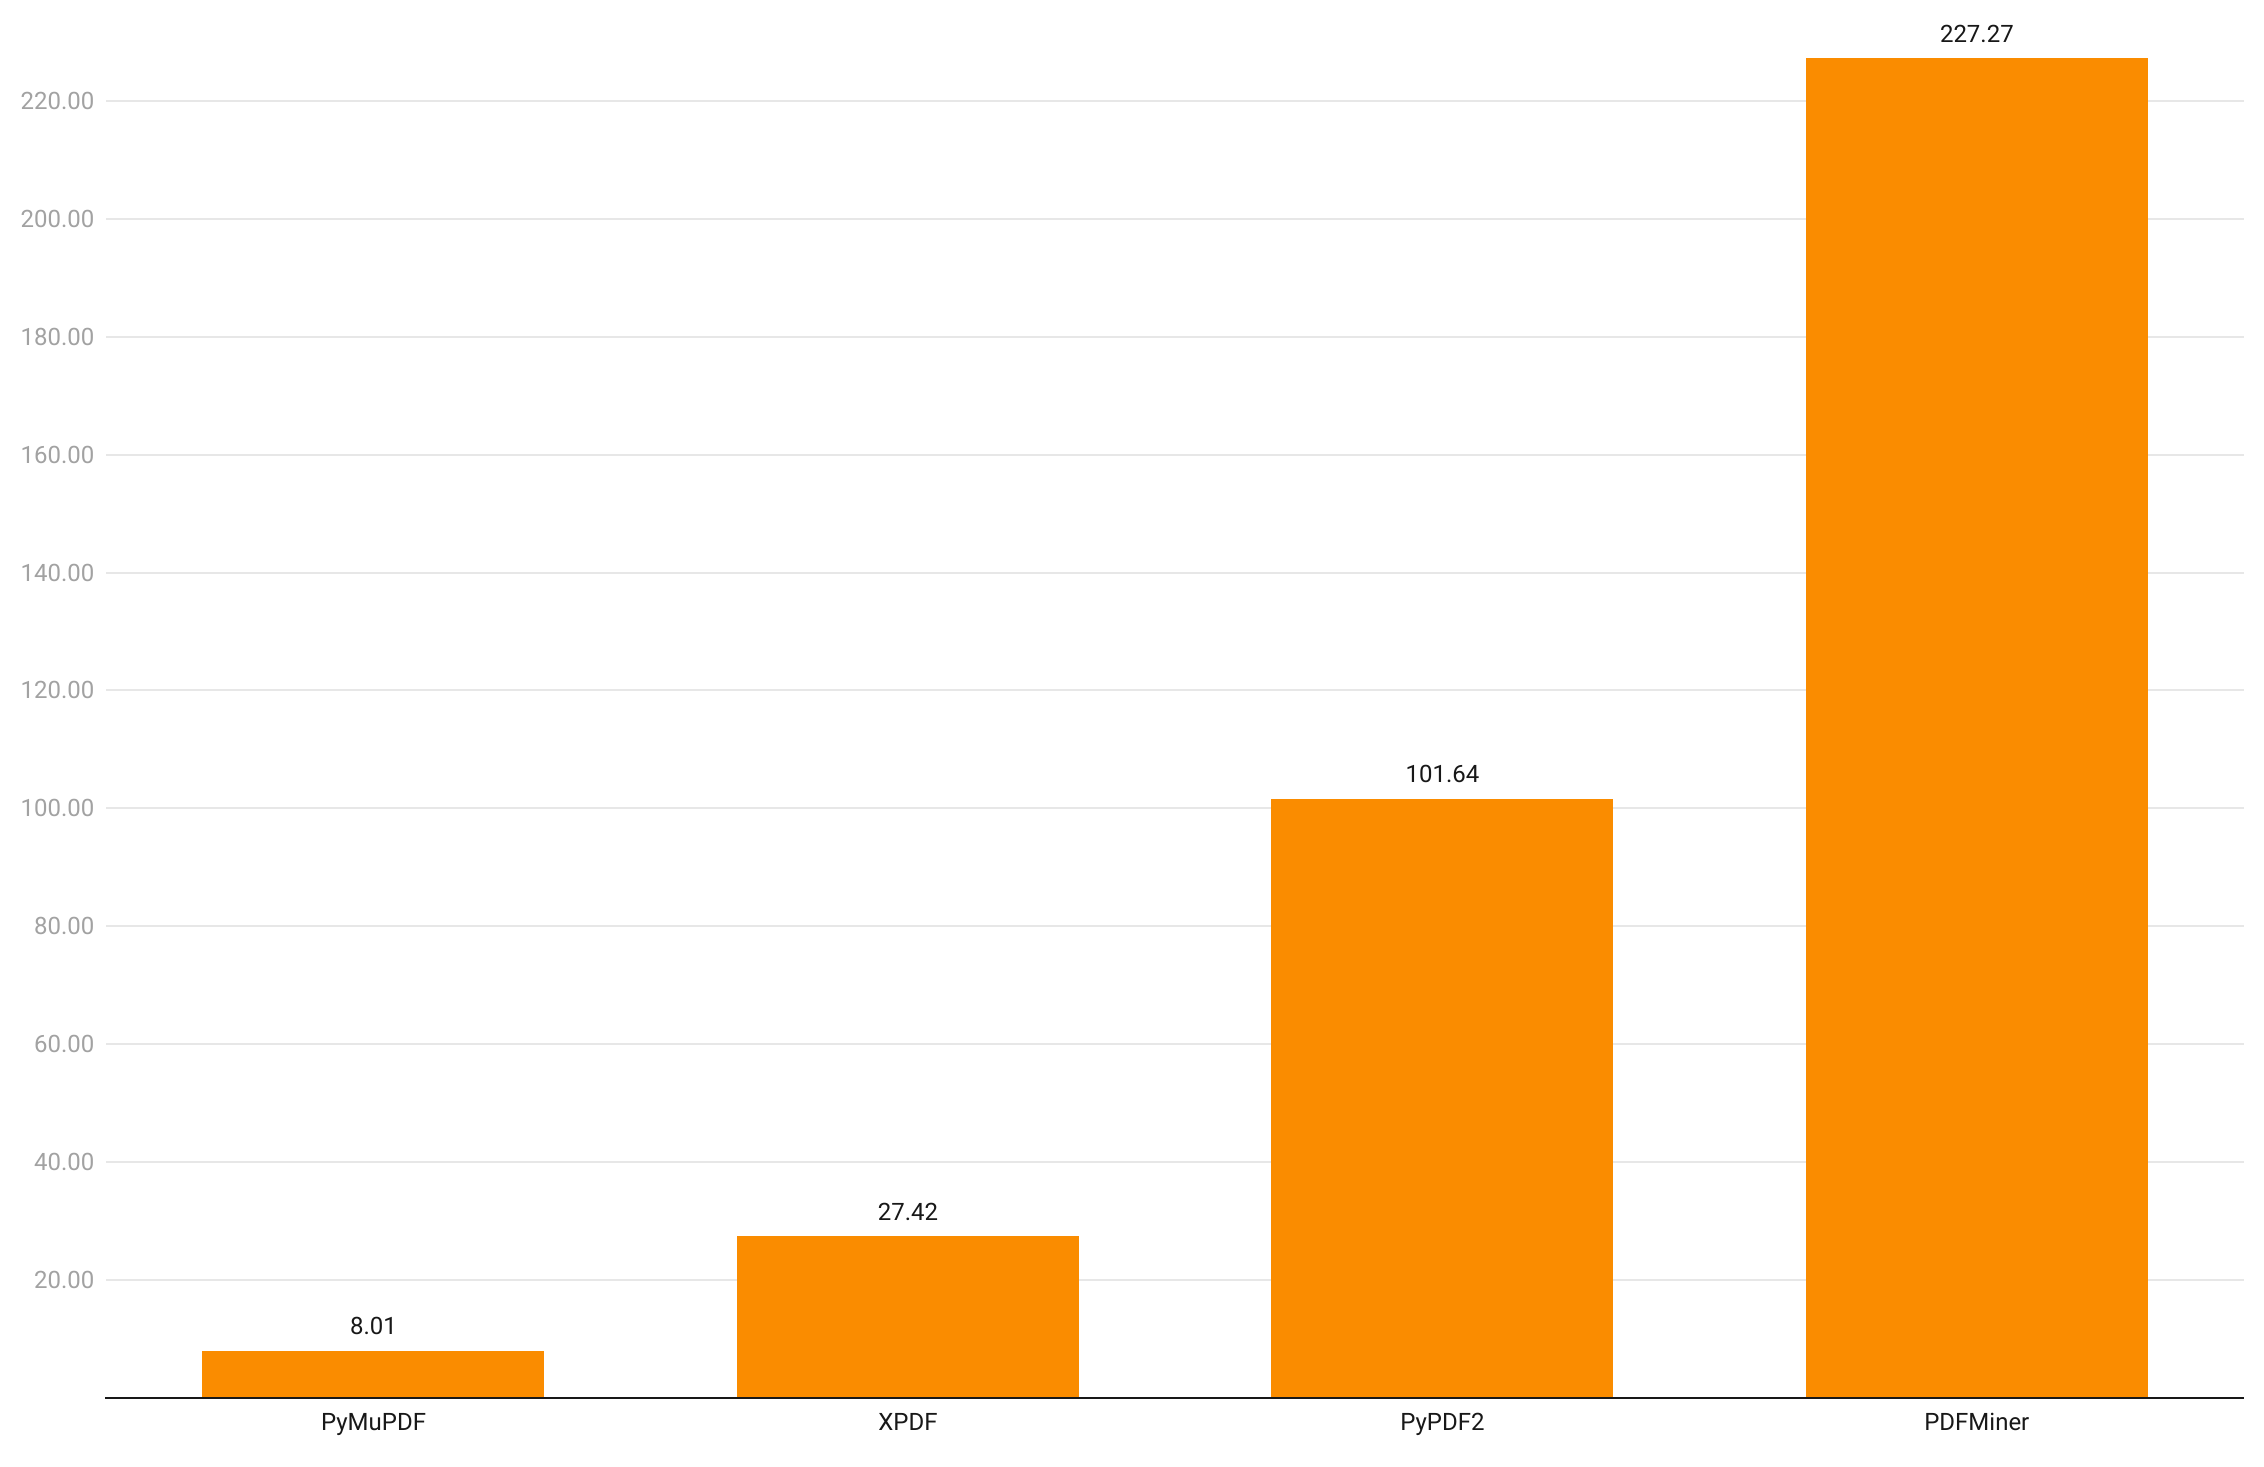
\includegraphics[scale=.25]{Figura3_2}
	\caption{Comparație de timp (în secunde) pentru extragerea textului din documente PDF}
	\label{fig:Figura3_2}
\end{figure}

Ultimul test măsoară viteza de transformare a documentelor PDF în imagini. Această funcționalitate este utilă atunci când se dorește afișarea paginilor din documentul PDF într-o interfață. Deschiderea unei imagini este mai rapidă decât deschiderea unui documentu. Rezultatele testului sunt afișate în figura 3.3.
\begin{figure}[H]
	\centering
	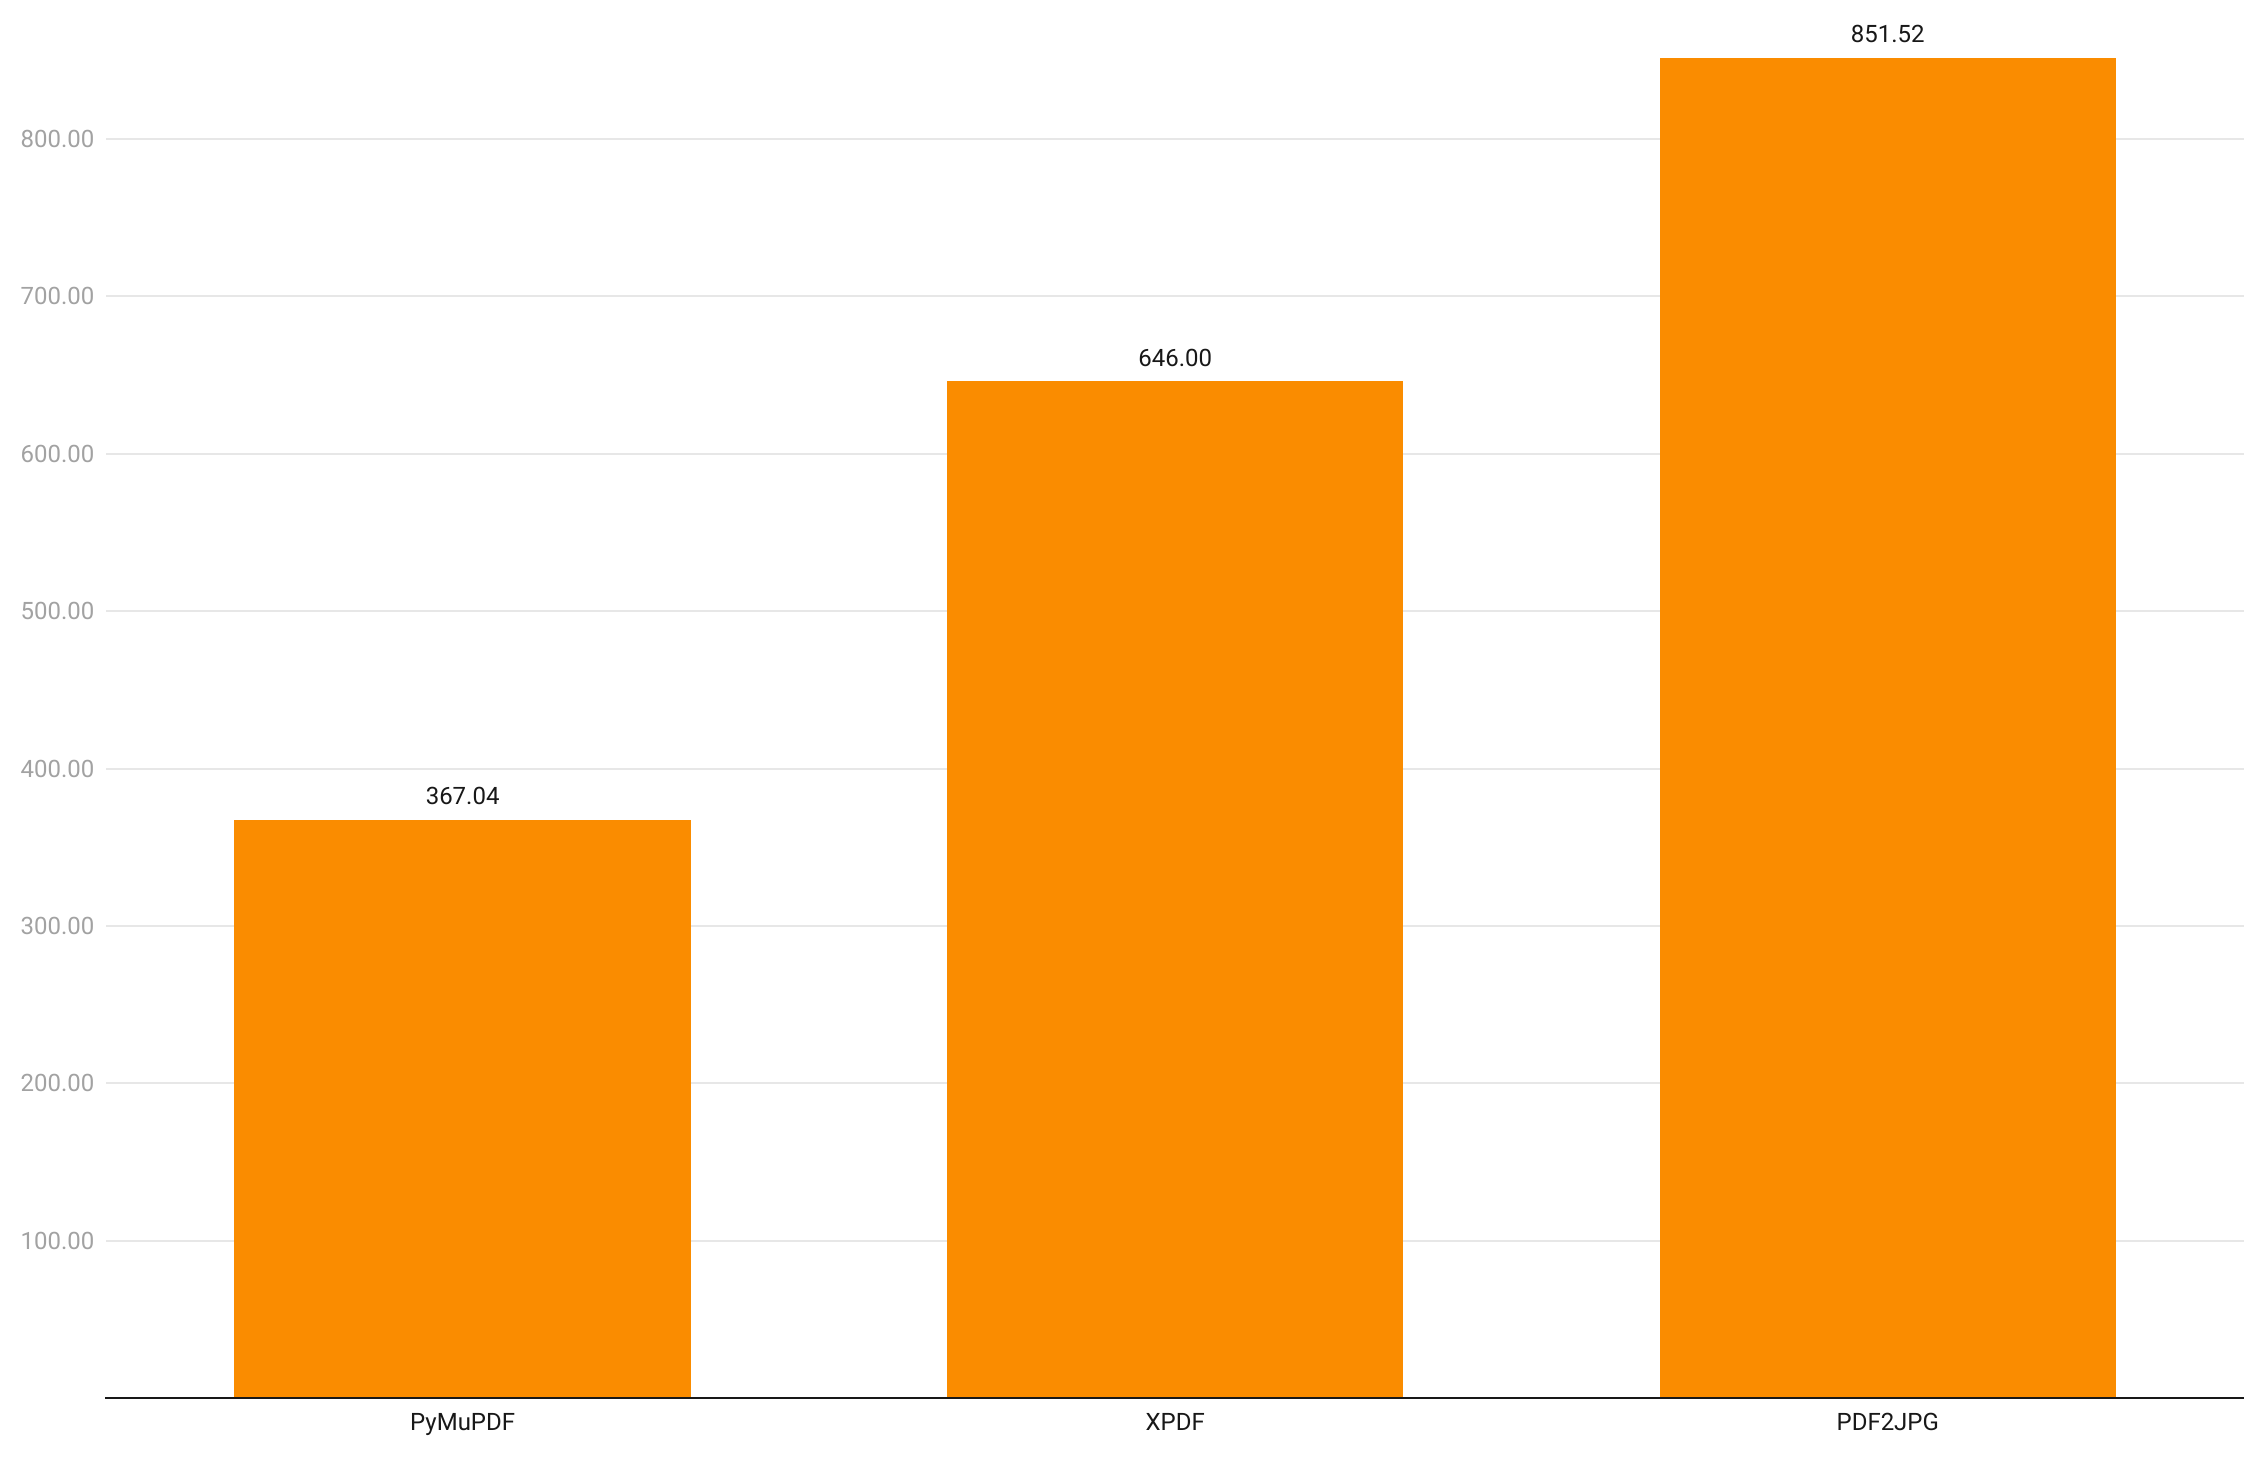
\includegraphics[scale=.2]{Figura3_3}
	\caption{Comparație de timp (în secunde) pentru transformarea paginilor în imagini}
	\label{fig:Figura3_3}
\end{figure}

Așa cum indică testele, PyMuPDF este o librărie de mare viteză care manipulează documente PDF. Pe lângă acest aspect, librăria oferă multe funcționalități și este constant actualizată. Din aceste motive, aplicația de automatizare va fi dezvoltată folosind PyMuPDF.


\section{MySQL}

MySQL \cite{dubois2013mysql} este un sistem de gestiune a bazelor de date (RDBMS). A fost lansat pe piață în anul 1995 de către MySQL AB. În anul 2008, compania a fost cumpărată de Sun Microsystems, iar aceștia în momentul de față fac parte din Oracle Corporation. MySQL este folosit de aplicații cunoscute precum: Facebook, Twitter, Netflix, Uber, Airbnb, Shopify.

Motivele principale pentru care a fost ales MySQL sunt ușurința integrării unei baze de date într-o aplicație dezvoltată în Python și viteza sa.  Rolul acestei baze de date în dezvoltarea aplicației de automatizare este de a stoca textul și metadatele din documentul PDF.




